\documentclass[14pt,t,aspectratio=169]{beamer}
\usepackage{fontspec}
\usepackage{color}
\usepackage{minted}
\usepackage{array}

%% These fonts are non-free.
%% Comment out the lines if you don't have them.
\setmainfont{Equity Text A}
\setsansfont{Concourse T3}
\setmonofont{Triplicate T4}

\definecolor{bgcolor}{RGB}{20,25,28}
\definecolor{codecolor}{RGB}{249,38,114}
\hypersetup{colorlinks,linkcolor=,urlcolor=codecolor}
\setbeamercolor{background canvas}{bg=bgcolor}
\setbeamercolor{normal text}{fg=white}
\setbeamercolor{itemize item}{fg=lightgray}
\setbeamercolor{enumerate item}{fg=lightgray}
\setbeamertemplate{itemize items}[circle]
\setbeamertemplate{navigation symbols}{}
%% These styles are kinda annoying the fuck outta me
%% If I have a change of heart (again), then here's the
%% file to edit:
%% /usr/lib/python3.6/site-packages/pygments/styles/monokai.py
%% Don't forget to remove the _minted* dir afterwards.
\usemintedstyle{monokai}
\newminted[lispcode]{common-lisp}{fontsize=\footnotesize}
\newminted[smalllispcode]{common-lisp}{fontsize=\scriptsize}
\def\code#1{{\color{codecolor}\texttt{#1}}}

\renewcommand{\theFancyVerbLine}{\color{darkgray}\large \oldstylenums{\arabic{FancyVerbLine}}}
\renewcommand{\title}[1]{
  {\huge #1} \vskip 0.4cm
}
\renewcommand{\subtitle}[1]{
  \vskip 0.3cm {\Large #1} \vskip 0.2cm %
}

\begin{document}
\begin{frame}
  \begin{center}
    
\includegraphics[width=\textwidth]{logo.png}\\
    \vspace{0.2cm}
    {\LARGE Nicolas Hafner} \\
    \vspace{0.2cm}
    {\Large @Shinmera} \\
    \vspace{0.2cm}
    \url{https://shinmera.com}
    \url{https://shirakumo.org}
  \end{center}
\end{frame}

\begin{frame}
  \title{About me}
  \begin{itemize}
  \item Founder of Shirakumo
  \end{itemize}
  \vfill
  
\includegraphics[width=\textwidth]{logo.png}
\end{frame}

\begin{frame}
  \title{About me}
  \begin{itemize}
  \item Founder of Shirakumo
  \item Open source maintainer
  \end{itemize}
  \vfill
  \centering
  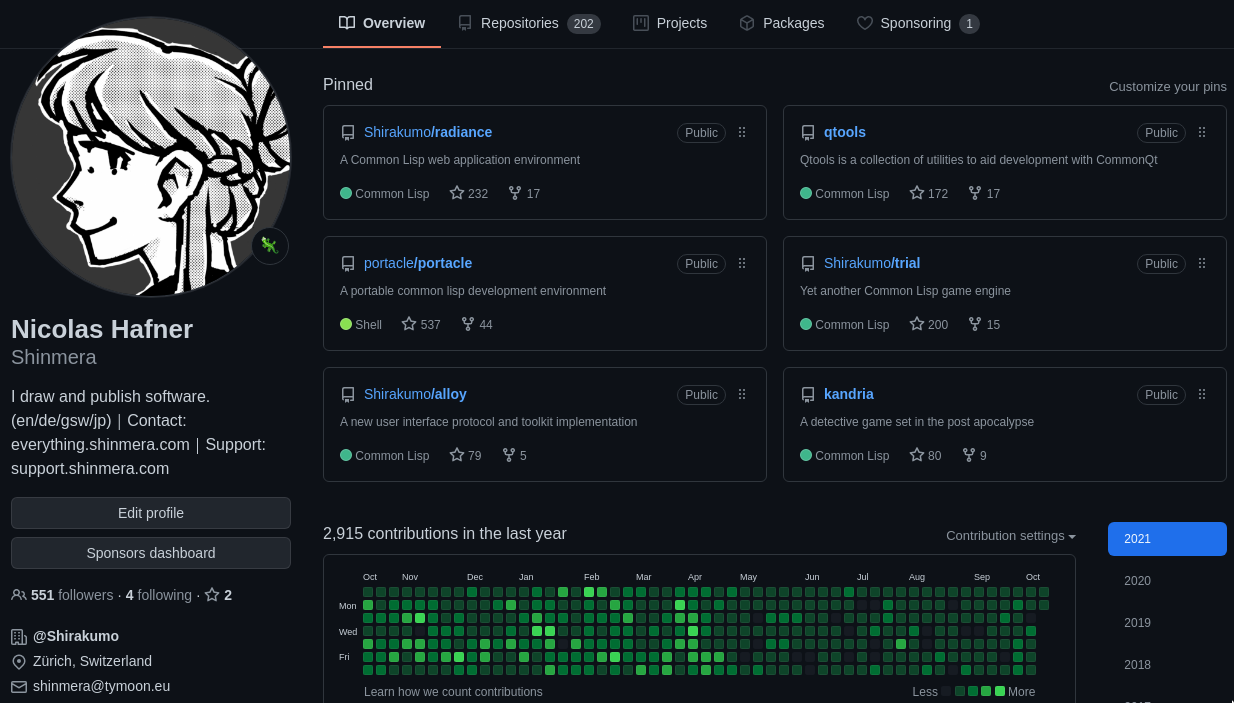
\includegraphics[width=0.8\textwidth]{github.png}
\end{frame}

\begin{frame}
  \title{About me}
  \begin{itemize}
  \item Founder of Shirakumo
  \item Common Lisp library maintainer
  \item Artist, etc.
  \end{itemize}
  \vfill
  
\includegraphics[width=\textwidth]{art.png}
\end{frame}

\begin{frame}
  \title{Background}
  \begin{itemize}
  \item Trial game engine and Kandria
  \item Full-stack lisp development
  \item Shipped Eternia: Pet Whisperer on PC
  \end{itemize}
  \vfill
  \centering
  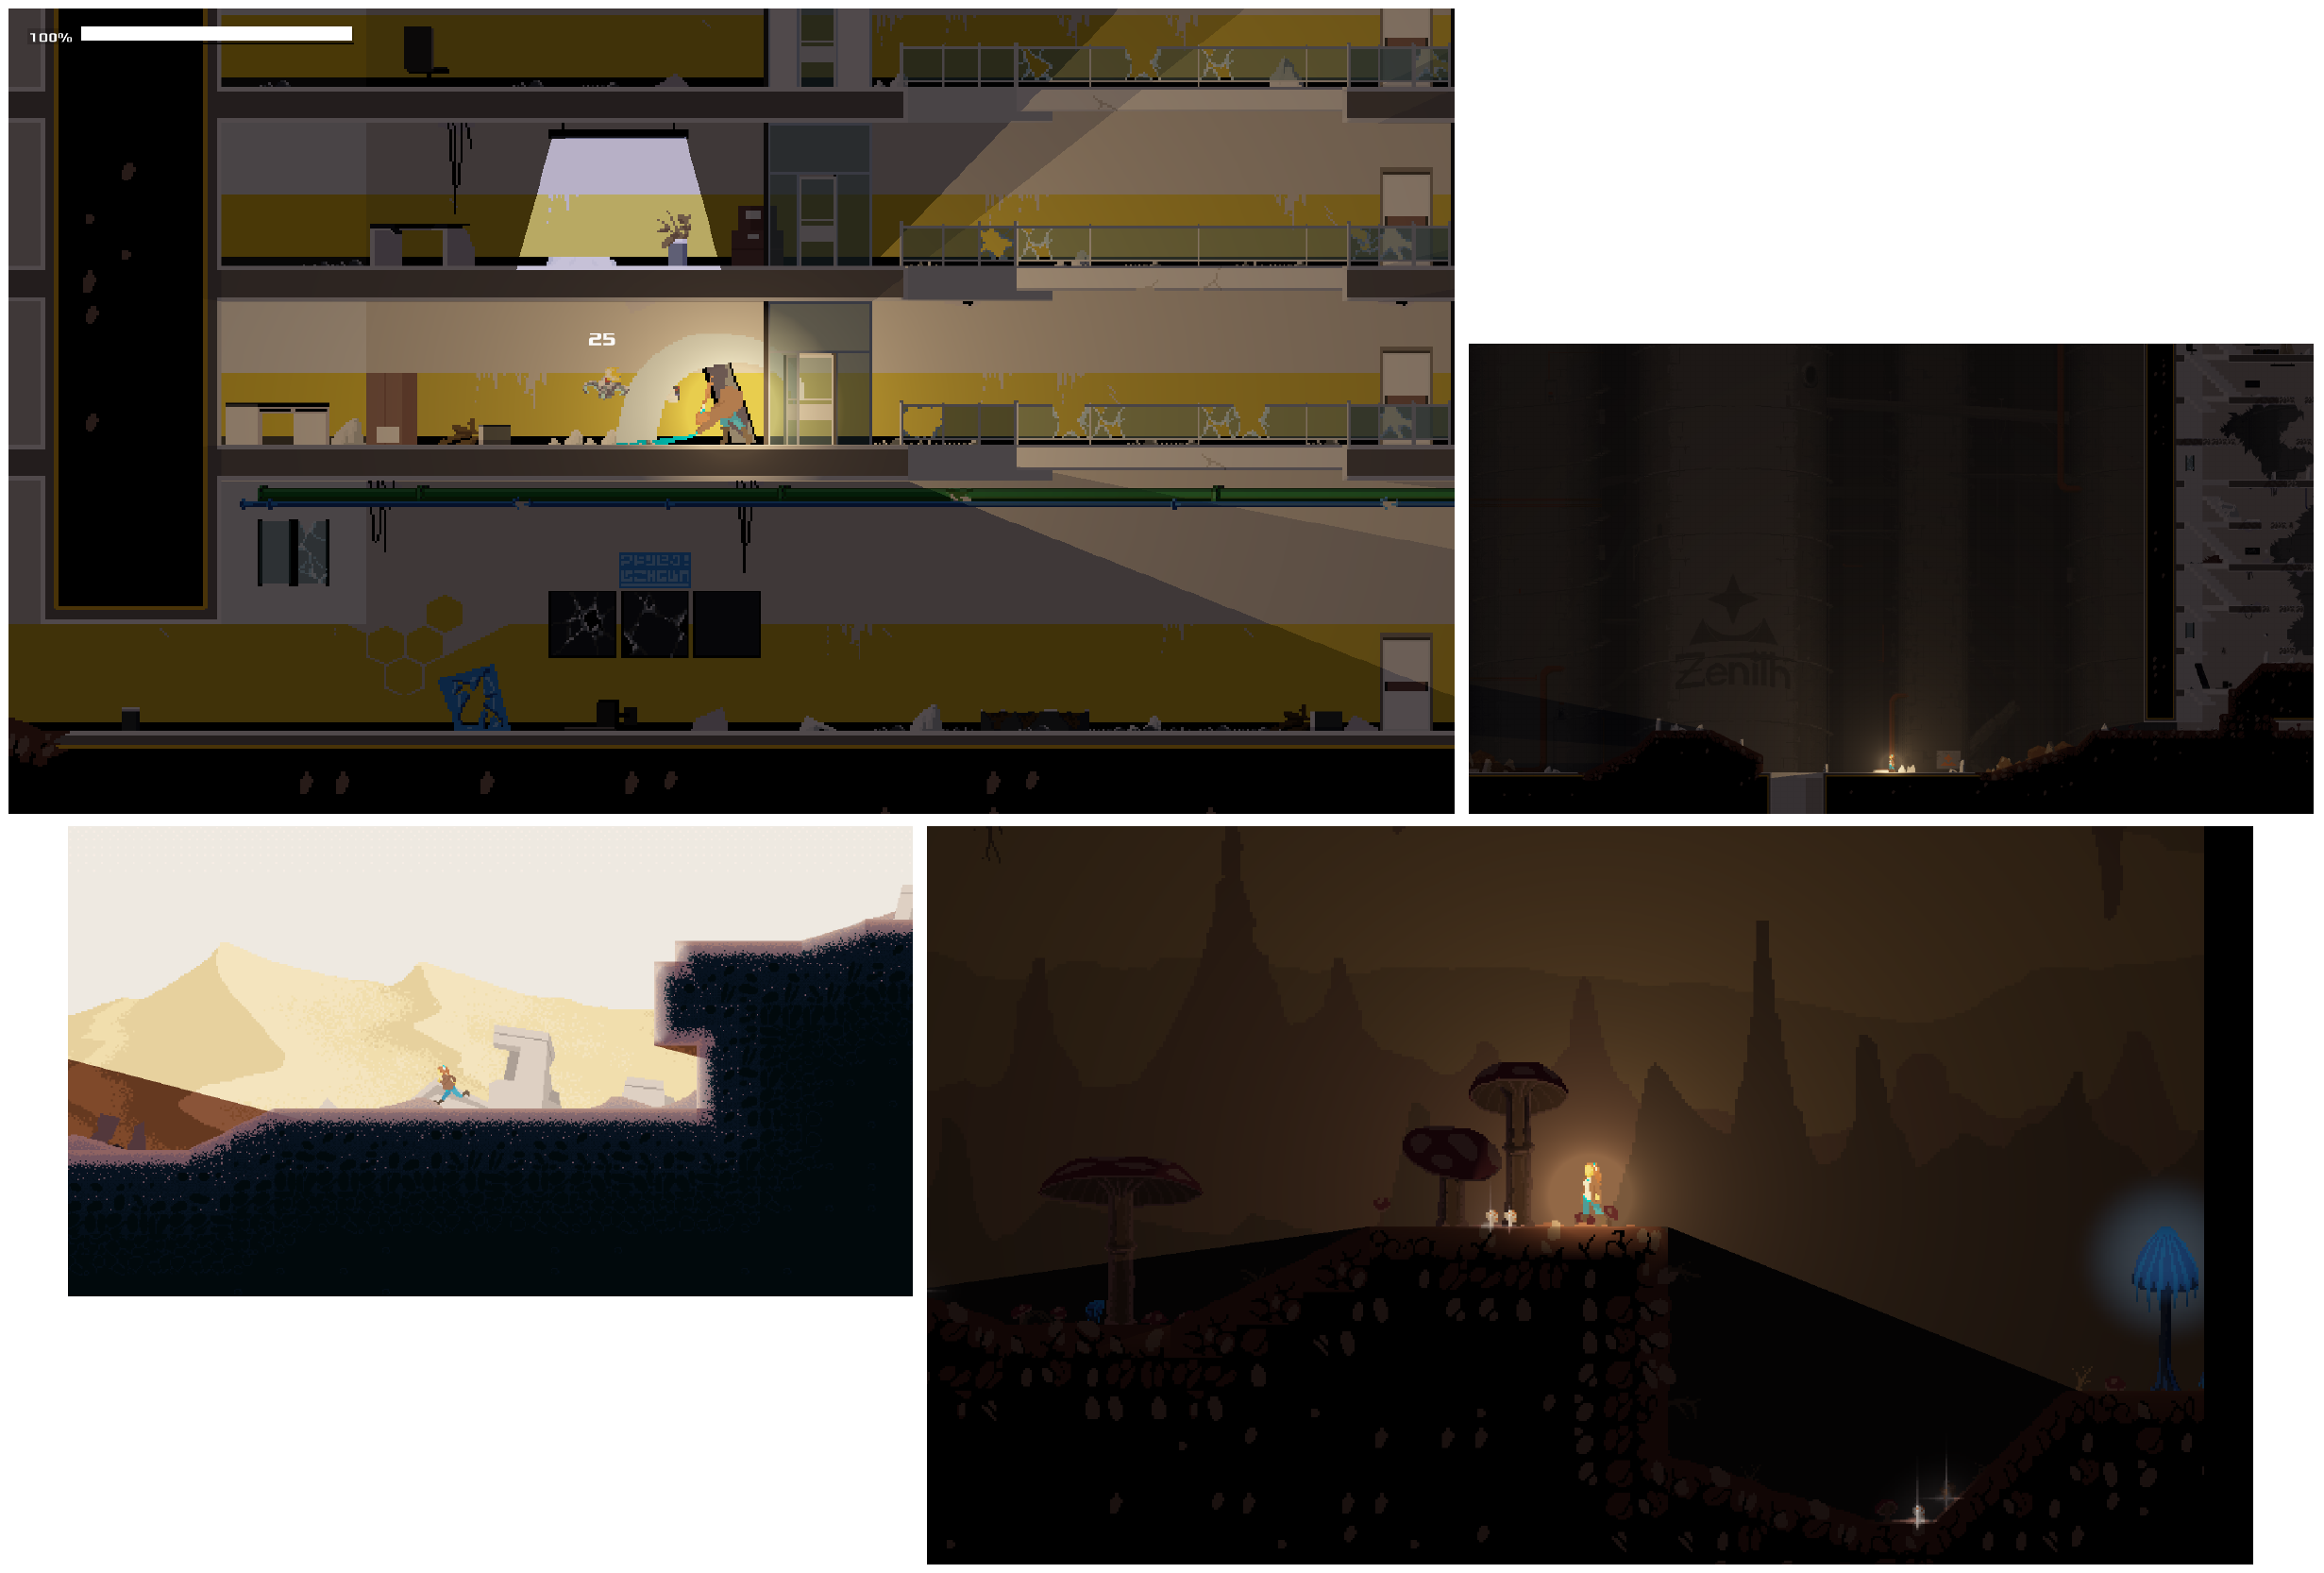
\includegraphics[width=0.7\textwidth]{screenshot.png}
\end{frame}

\begin{frame}
  \title{Why Common Lisp}
  \begin{itemize}
  \item Dynamic nature attractive for game iteration
  \item CLOS protocol design very comfortable
  \item Restarts great for interactive development
  \item Can change game entirely \textit{while it's running}
  \end{itemize}
  \pause\vfill
  We'll look at:
  \begin{itemize}
  \item Mixins / CLOS
  \item Restarts
  \item Optimization
  \item Garbage Collection
  \end{itemize}
\end{frame}

\begin{frame}
  \title{Mixins / CLOS}
  \begin{itemize}
  \item Encapsulate behaviours into small classes
  \item Generic functions + mixins comparable to ECS
  \item Fully runtime redefinable
  \item Can even change class of an existing instance (!)
  \end{itemize}
\end{frame}

\begin{frame}[fragile]
  \title{Mixins / CLOS}
\begin{lispcode}
(defclass event () ())
(defclass tick (event) ())

(defclass entity () ())
(defclass player (entity) ())
(defclass enemy (entity) ())

(defgeneric handle (event object))
\end{lispcode}
\end{frame}

\begin{frame}[fragile]
  \title{Mixins / CLOS}
\begin{lispcode}
;; Catch-all
(defmethod handle ((event tick) (object entity)))

;; Player input handling
(defmethod handle ((event tick) (object player))
  (print :player)
  (when (pressed :left) ...)
  (when (pressed :right) ...))

;; Enemy AI logic
(defmethod handle ((event tick) (object enemy))
  (print :enemy)
  (when (see 'player) ...))

;; Sample call
(handle tick enemy)
=> :enemy
\end{lispcode}
\end{frame}

\begin{frame}[fragile]
  \title{Mixins / CLOS}
\begin{lispcode}
;; A new emitter class with a flickering light
(defclass emitter () ())

(defmethod handle :after ((event tick) (object emitter))
  (print :emitter)
  (update-intensity ...))
\end{lispcode}
  \pause\vspace{0.5cm}
\begin{lispcode}
;; Update the class ↓
(defclass enemy (emitter entity) ())

;; Sample call
(handle tick enemy)
=> :enemy :emitter
\end{lispcode}
\end{frame}

\begin{frame}[fragile]
  \title{Mixins / CLOS}
  An example from our actual code-base
  \vspace{0.5cm}
\begin{lispcode}
(defclass player (alloy:observable stats-entity
                  paletted-entity animatable
                  profile ephemeral inventory)
  (...))
\end{lispcode}
  \pause\vspace{0.5cm}
\begin{lispcode}
(length (compute-class-precedence-list 'player))
=> 32
\end{lispcode}
\end{frame}

\begin{frame}
  \title{Problems}
  \begin{itemize}
  \item Class order can have surprising consequences
  \item Protocols need to be carefully designed
  \item Dispatch overhead can be significant
  \end{itemize}
\end{frame}

\begin{frame}
  \title{Restarts}
  \begin{itemize}
  \item Specify ways to recover from errors
  \item Debugger can then use restarts to continue
  \item Surrounding dynamic context can do this, too
  \end{itemize}
  \pause
  \vspace{0.5cm}
  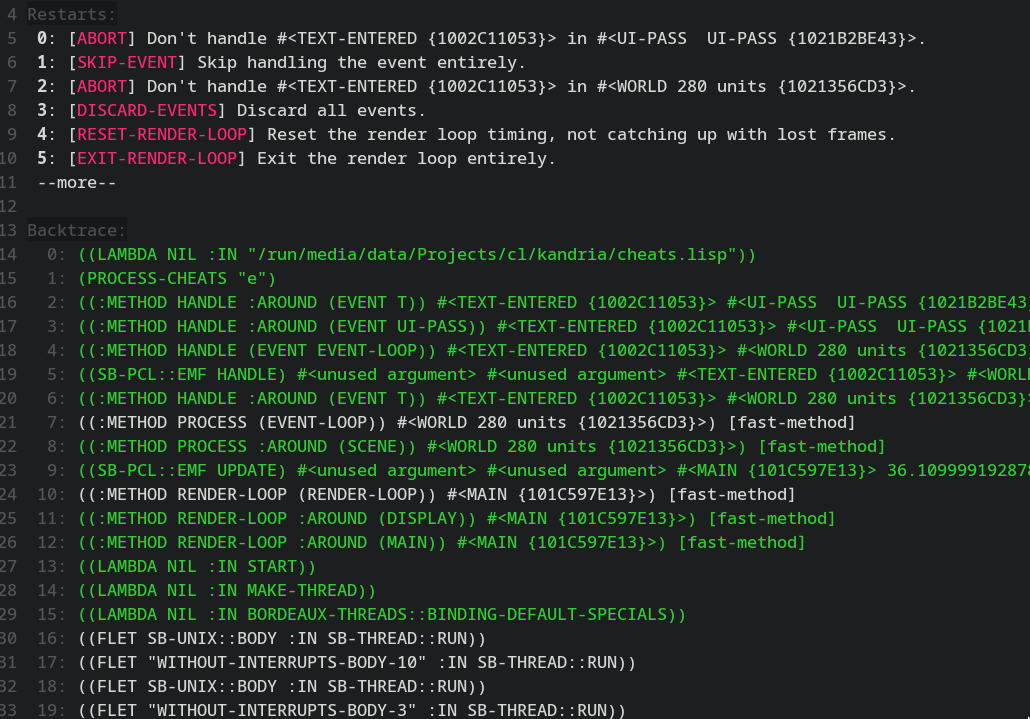
\includegraphics[width=\textwidth]{debugger.png}
\end{frame}

\begin{frame}[fragile]
  \title{Restarts}
\begin{lispcode}
(defmethod render :around (object target)
  (restart-case (call-next-method)
    (abort ())
    (retry ()
      (render object target))))
\end{lispcode}
\pause\vspace{0.5cm}
\begin{lispcode}
(defun main ()
  #+release
  (handler-bind ((error (invoke-restart 'abort)))
    (start-game))
  #-release
  (start-game))
\end{lispcode}
\end{frame}

\begin{frame}[fragile]
  \title{Restarts}
  \begin{itemize}
  \item Debugger pauses affected thread
  \item Can fix underlying problem while running
  \item Recompile anything, change any variable!
  \item Then resume from a fitting restart
  \end{itemize}
\end{frame}

\begin{frame}
  \title{Optimisation}
  \begin{itemize}
  \item Standard dynamic language issues apply
  \item Dynamic by default means indirection and checks
  \item Generic function dispatch overhead significant
  \end{itemize}
  \pause
  but...
  \begin{itemize}
  \item SBCL can infer a lot of type information
  \item Programmer can declare missing types
  \item Assembly of generated functions can be inspected
  \item Compiler is customisable from within Lisp
  \item New work being done to speed up dispatch (Strandh et al.)
  \end{itemize}
\end{frame}

\begin{frame}[fragile]
  \title{Optimisation}
\begin{lispcode}
(disassemble
  (lambda (x)
    (* x x)))
; disassembly for (LAMBDA (X))
; Size: 33 bytes. Origin: #x54A24624
; 24:       498B5D10         MOV RBX, [R13+16]
; 28:       48895DF8         MOV [RBP-8], RBX
; 2C:       488BD6           MOV RDX, RSI
; 2F:       488BFE           MOV RDI, RSI
; 32:       FF14251801A052   CALL QWORD PTR [#x52A00118]
; 39:       488B75F0         MOV RSI, [RBP-16]
; 3D:       488BE5           MOV RSP, RBP
; 40:       F8               CLC
; 41:       5D               POP RBP
; 42:       C3               RET
; 43:       CC10             INT3 16
\end{lispcode}
\end{frame}

\begin{frame}[fragile]
  \title{Optimisation}
\begin{lispcode}
(disassemble
  (lambda (x)
    (declare (type (unsigned-byte 16) x))
    (declare (optimize speed (safety 0)))
    (* x x)))
; disassembly for (LAMBDA (X))
; Size: 16 bytes. Origin: #x5365AB36
; 36:       48D1FA           SAR RDX, 1
; 39:       480FAFD2         IMUL RDX, RDX
; 3D:       48D1E2           SHL RDX, 1
; 40:       488BE5           MOV RSP, RBP
; 43:       F8               CLC
; 44:       5D               POP RBP
; 45:       C3               RET
\end{lispcode}
\end{frame}

\begin{frame}
  \title{Garbage collection}
  \begin{itemize}
  \item Dynamic languages need a GC
  \item SBCL provides a generational compacting GC
  \item GC pauses \textit{are} a problem
  \item Pauses are stop-the-world, single-threaded
  \end{itemize}
  \pause\vfill
  but...
  \begin{itemize}
  \item Problem can be mitigated with standard tech:
  \item Object pooling, static allocation, immutability
  \item Thanks to macros, boilerplate can be hidden!
  \end{itemize}
\end{frame}

\begin{frame}[fragile]
  \title{Garbage collection}
\begin{lispcode}
(defun color (r g b)
  (make-instance 'color r g b))

(define-compiler-macro color (r g b &whole form)
  (if (and (constantp r)
           (constantp g)
           (constantp b))
      `(load-time-value (make-instance 'color ,r ,g ,b))
      whole))
\end{lispcode}
  \pause\vspace{0.5cm}
\begin{lispcode}
(color 1.0 1.0 1.0)
=> (load-time-value (make-instance 'color 1.0 1.0 1.0))
\end{lispcode}
\end{frame}

\begin{frame}
  \title{Conclusions}
  \begin{itemize}
  \item Significant challenges exist
  \item Effort has to be put in to optimise...
  \item especially regarding vectorisation and garbage
  \item Proper design is important and takes time
  \end{itemize}
  \pause\vfill
  but...
  \begin{itemize}
  \item Often the development speed benefits outweigh
  \item Iteration much faster with runtime recompilation
  \item The capabilities are all there
  \end{itemize}
\end{frame}

\begin{frame}
  \title{Paper available}
  \begin{tabular}{m{5cm}m{10cm}}
    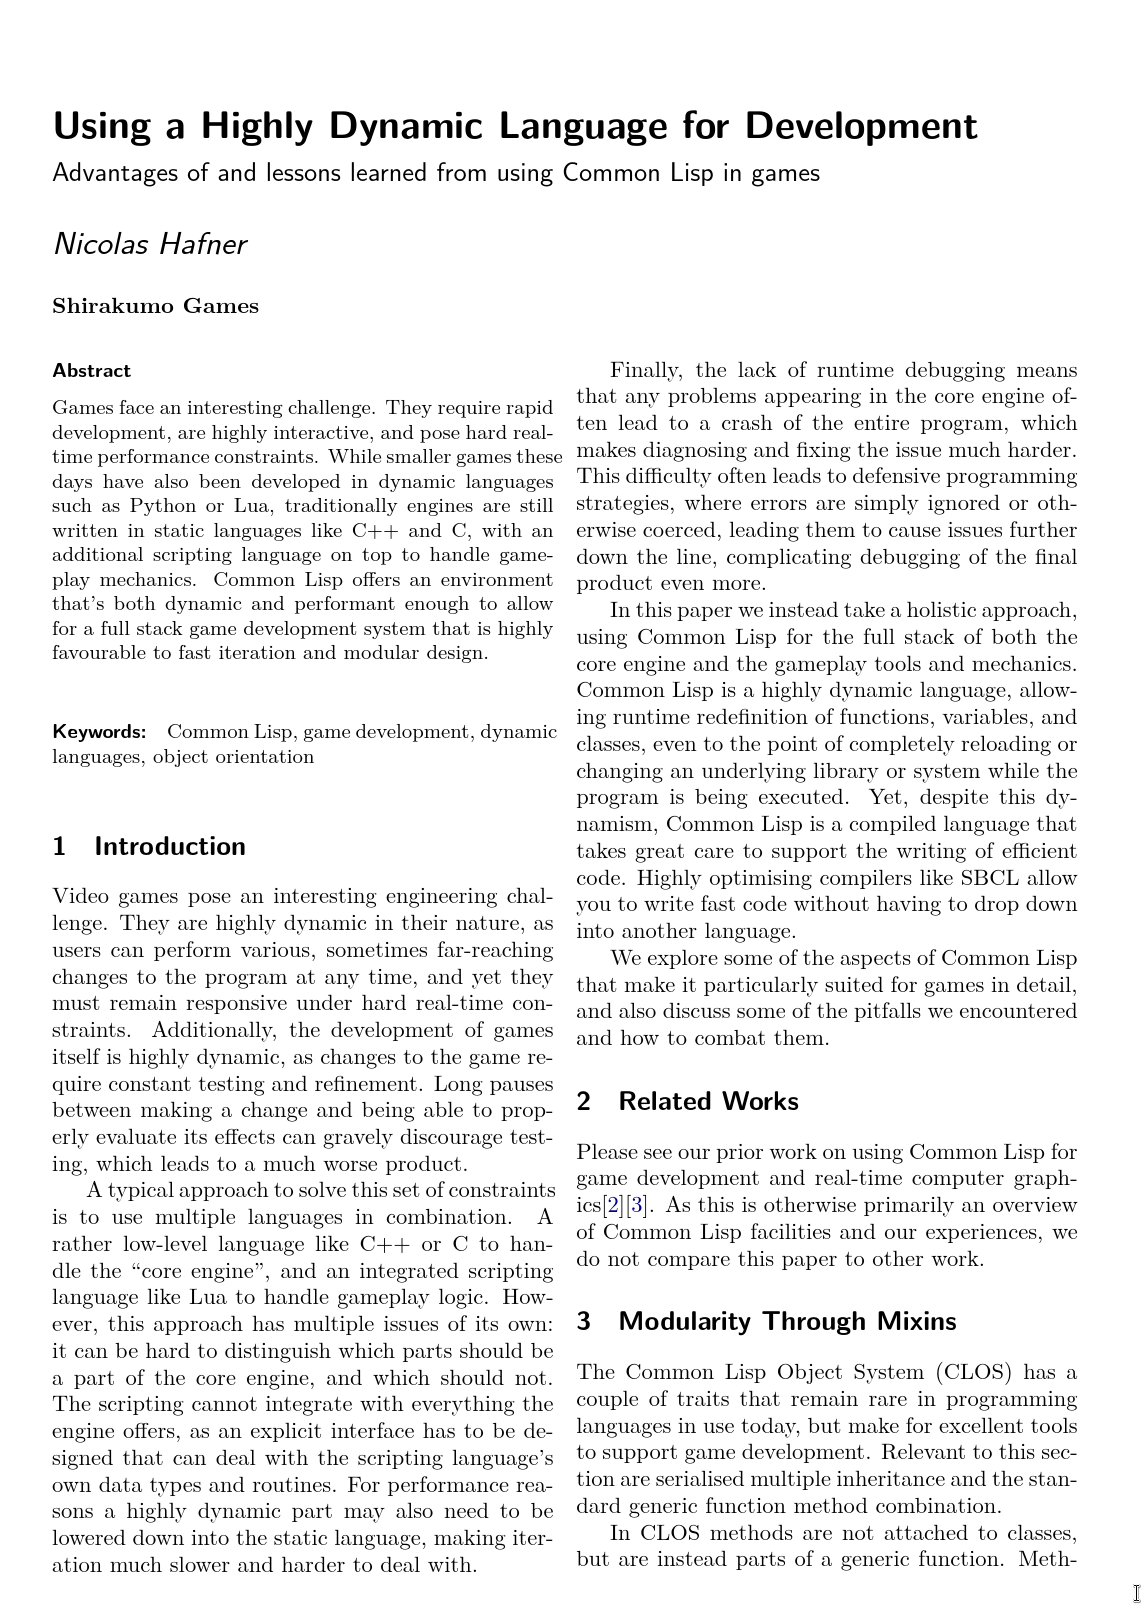
\includegraphics[width=5cm]{paper.png} & \url{shinmera.com/paper/gic21.pdf}
  \end{tabular}
\end{frame}

\begin{frame}
  \title{Thanks for listening!}
  \centering
  
\includegraphics[width=0.8\textwidth]{main capsule.png} \\
  \url{https://kandria.com}
\end{frame}

\end{document}

%%% Local Variables:
%%% mode: latex
%%% TeX-master: t
%%% TeX-engine: luatex
%%% TeX-command-extra-options: "-shell-escape"
%%% End:
